\section{Historical Context}

The synthesis of materials by alkali activation began in the 1930s and 1940s, when a substitute for traditional Portland cement was developed from blast furnace slag and other aluminosilicates \cite{pachecotorgal2014handbook}.
From the 1970s onwards, interest in this area increased, when the French scientist Joseph Davidovits coined the term "geopolymer" and patented several formulations. His initial studies focused on the development of inorganic, non-flammable, and fire-resistant materials \cite{provis2009geopolymers}.

%% There is another article important here that you may cite

Since then, alkali-activated materials (AAM) have attracted the attention of researchers and industry due to their low energy consumption and sustainable nature \cite{qin2022onepart}.
Furthermore, as studies have advanced, AAMs have gained recognition for their mechanical properties and durability, as the polymerization reactions that occur during curing provide high compressive strength and resistance to chemical attack.

%% Differenciate AAM from geopolymers

While the term alkali-activated materials broadly refers to binders produced through the reaction of aluminosilicate sources with alkaline activators, the term geopolymer defines a narrower class within this family.
The distinction between them lies in both composition and reaction mechanisms, as depicted in Figure \ref{fig:al_ca_aam}.
AAMs may include calcium-rich precursors, whereas geopolymers represent the low-calcium end of the alkaline activation spectrum.

\begin{figure}[H]
  \centering
  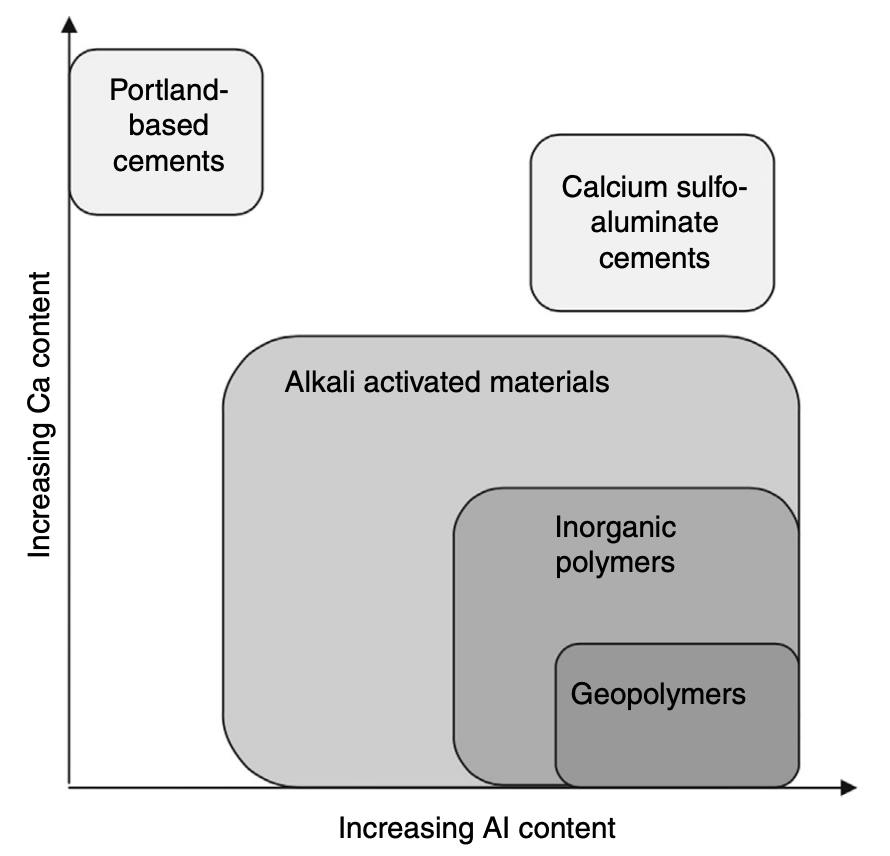
\includegraphics[width=0.5\textwidth]{Cap2/images/al_ca_aam.png}
  \caption{Classification of different subsets of alkali-activated materials, with comparisons to Portland cement and
calcium sulfoaluminate binder chemistry. Shading
indicates approximate alkali content; darker shading
corresponds to higher concentrations of Na and/or K \cite{rakhimova2019reaction}.}
  \label{fig:al_ca_aam}
\end{figure}


\section{Raw Materials for AAM}

\subsection{Solid Precursors}

Precursors are materials rich in $SiO_2$ and $Al_2O_3$ that, when activated by an alkaline solution, form a three-dimensional network of aluminosilicates \cite{rakhimova2019metakaolin}.
The chemical mechanisms of AAMs are strongly influenced by the $SiO_2/Al_2O_3$ ratio \cite{provis2007geopolymerisation}.
The initial activation process involves the dissolution of aluminosilicates through the breaking of covalent bonds $Si-O-Si$ and $Al-O-Al$ in a high pH environment \cite{Severo2013}. Hydrolysis can be represented as follows:

\begin{equation}
  Al_2O_3 + 3H_2O + 2OH^- \rightarrow 2\left[Al(OH)_4\right]^- 
\end{equation}

\begin{equation}
  SiO_2 + H_2O + OH^- \rightarrow \left[SiO(OH)_3\right]^- 
\end{equation}

\begin{equation}
  SiO_2 + 2OH^- \rightarrow \left[SiO_2(OH)_2\right]^{2-}
\end{equation}

Subsequently, the dissolved silicates and aluminates react with each other, forming a gel that undergoes polymerization and hardening processes, as illustrated in Figure \ref{fig:activation}.

\begin{figure}[ht]
  \centering
  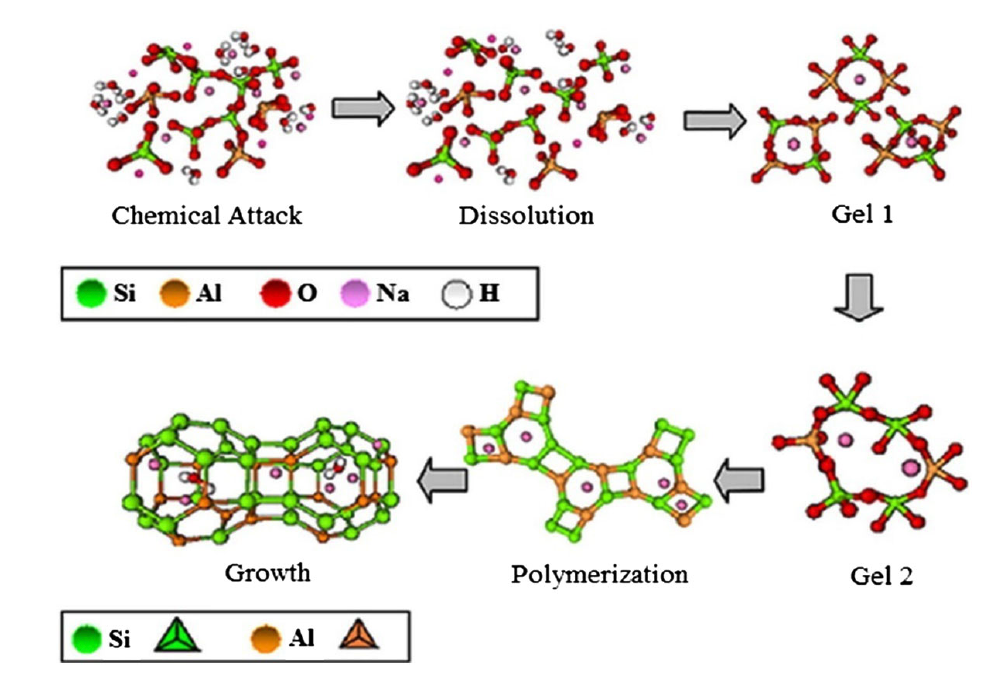
\includegraphics[width=0.75\textwidth]{Cap2/images/activation.png}
  \caption{Scheme of the alkaline activation process \cite{duxson2006geopolymer}.}
  \label{fig:activation}
\end{figure}

Precursors can be divided into two categories: those with high calcium content, such as blast furnace slag and fly ash, and those with low calcium content, such as metakaolin.
Figure \ref{fig:ternary_diagram} shows the most common precursors and their respective chemical compositions.

\begin{figure}[ht]
  \centering
  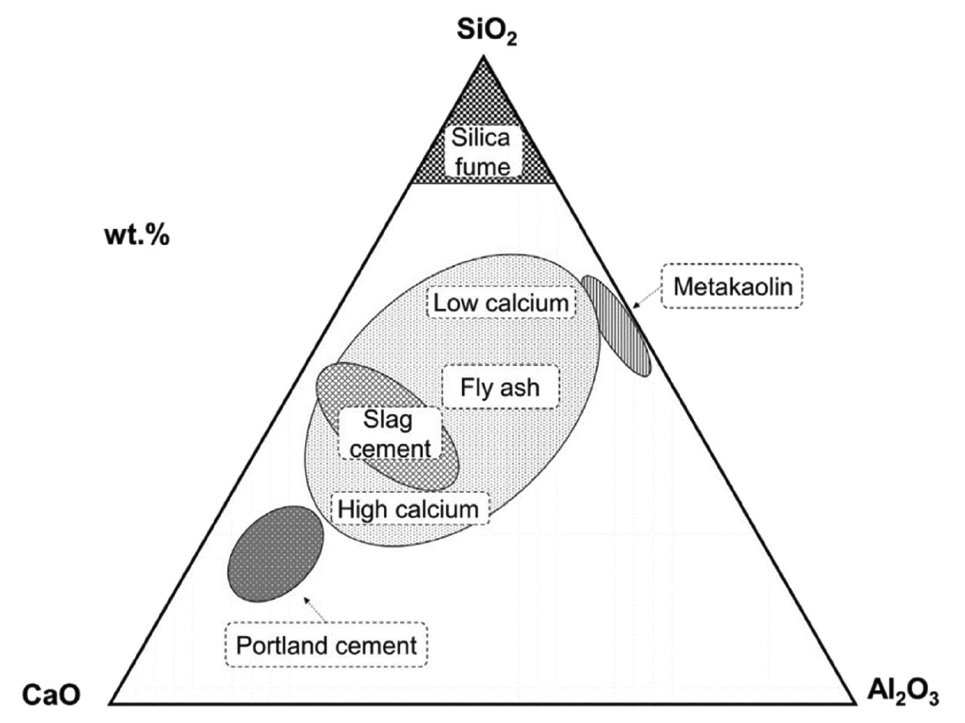
\includegraphics[width=0.625\textwidth]{Cap2/images/ternary_diagram.png}
  \caption{Ternary diagram of the most common precursors \cite{giergiczny2019fly}.}
  \label{fig:ternary_diagram}
\end{figure}

The first group primarily produces calcium aluminate silicate hydrate (C-A-S-H) as a result of the activation reaction, while the second group predominantly forms sodium aluminosilicate hydrate (N-A-S-H) gel.

When the calcium levels in these precursors are high, the final product is a gel with rapid curing and high initial strength. However, these systems are more susceptible to shrinkage, cracking, and corrosion due to chloride attack.
On the other hand, low-calcium systems form an tetrahedrical amorphous network, which exhibits low permeability and shrinkage, better fire resistance, and a less porous structure.
The $SiO_2/Al_2O_3$ ratio is responsible for the degree of polymerization of the formed gel; therefore, if the ideal ratio is not achieved, the mechanical strength and durability of the AAM may be compromised.
Finally, the N-A-S-H gel requires a longer curing time and a temperature between $80-100\ ^\circ C$ to reach the appropriate mechanical strength \cite{Nodehi2021}.

Table \ref{tab:common_precursors} presents the main characteristics of the most common precursors.

\begin{landscape}
\begin{table}[p]
  \centering
  \caption{Characteristics of common or innovative residual materials that can be added to concrete to produce more sustainable binders \cite{Nodehi2021}.}
  \vspace{0.5cm}
  {\small % Reduce font size for the table
  \renewcommand{\arraystretch}{1.2} % Increase row spacing
  \begin{tabular}{p{3.5cm} p{3cm} p{2cm} p{2cm} p{4cm} p{6cm}}
    \hline
    Additive name & Usual form & Average density (kg/m\textsuperscript{3}) & Average particle size (\textmu m) & Limitations & Benefits \\
    \hline
    Silica fume & Spherical & 2200 & 0.1--0.5 & Reduces workability and initial strength & Increases compactness, mechanical strength, and durability \\
    Ground granulated blast furnace slag (GGBFS) & Angular with rough surface & 1000--1300 & 1.25--250 & Low initial strength & Increases durability, improves ITZ, and sulfate resistance \\
    Fly ash & Spherical & 540--860 & 0.5--300 & Low initial strength & Improves workability and long-term strength \\
    Metakaolin & Porous, lamellar, and angular & 890 & 1--20 & Reduces workability & Fills microstructure and improves ITZ \\
    Rice husk ash & Irregular with high porosity & 504--700 & 5--10 & Property variation and low reactivity & High silica content; improves compactness and strength \\
    Glass powder & Irregular & 2500 & 0.8--50 & High contamination & Improves durability and pozzolanic reaction \\
    Red mud & Irregular and needle-shaped & 2700--3400 & 100 to over 200 & High contamination & High alumina content, can improve hydration \\
    Ceramic waste & Angular & ~1700 & Below 100 & -- & Improves compactness and performance \\
    Municipal solid waste incineration slag (MSWI) & Irregular & 660--1690 & -- & -- & Improves microstructure and reduces porosity \\
    Paper sludge ash & Irregular & Below 100 & -- & -- & Favourably adjusts the S/A ratio \\
    \hline
  \end{tabular}
  }
\label{tab:common_precursors}
\end{table}
\end{landscape}

% \subsubsection{Metakaolin}

% \subsubsection{Silica Fume}

\subsection{Activators}

The alkaline attack on the microstructure of the precursors results in the release of silicates and aluminates into the solution.
The solubility of silica and alumina as a function of pH is presented in Figure \ref{fig:solubility}.

\begin{figure}[ht]
  \centering
  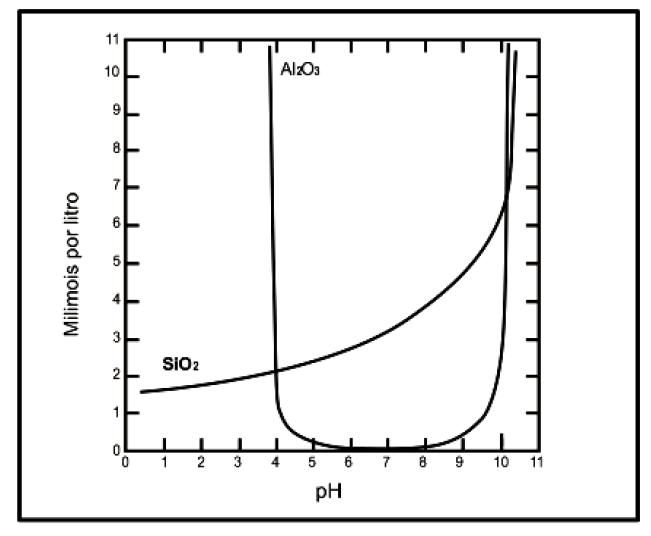
\includegraphics[width=0.625\textwidth]{Cap2/images/solubility.png}
  \caption{Solubility of silica and alumina as a function of pH \cite{mason1952principles}.}
  \label{fig:solubility}
\end{figure}

It is observed that the solubility of silica is low in acidic environments and high in basic media, while alumina is soluble at both extremes of pH.
Therefore, for the activation reactions to occur, it is necessary that the pH of the solution is high.

Alkaline activators can be found in two forms: liquid—producing two-part geopolymers—or solid—one-part geopolymers.
The main liquid alkaline activators are: sodium hydroxide ($NaOH$), sodium silicate ($Na_2SiO_3$), potassium hydroxide ($KOH$), sodium carbonate ($Na_2CO_3$) and potassium carbonate ($K_2CO_3$).
The first studies on AAM focused on liquid activators, since the final product exhibits high compressive strength, adhesion, and the ability to withstand fatigue loads. In addition, they also demonstrate high resistance to freeze-thaw cycles and high temperatures \cite{heath2014gwp}.

Despite the advantages of two-part systems, basic solutions are corrosive and irritate human skin, making their transport and handling hazardous for workers \cite{awoyera2019critical}.
Another point worth noting is that the production of sodium silicate occurs between $1200-1400\ ^\circ C$ and emits approximately 1.514 kg of $CO_2$ per kg of silicate produced, in addition to significantly contributing to air pollution through dust and nitrogen and sulfur oxides \cite{rajan2020sustainable}.

Therefore, even in one-part alkali-activated systems, the use of hydroxides still poses a significant safety concern, as their corrosive nature is intrinsic to the chemical compound itself rather than to the activation method. Consequently, to enable the broader and safer application of one-part alkali-activated binders, it is essential to seek alternative alkaline sources that exhibit lower corrosivity while maintaining sufficient reactivity for effective activation.

\section{Environmental Impacts}

The main environmental advantage attributed to AAMs lies in the considerable reduction of $CO_2$ emissions compared to traditional Portland cement.
It is estimated that the environmental impacts of solid and liquid activators are 24\% and 60\% of the impact caused by OPC, respectively \cite{luukkonen2017review}.
Furthermore, the production of AAMs often utilizes industrial residues as raw materials, such as sewage sludge ash, sugarcane straw ash, among others \cite{moraes2024scsa}.
Therefore, in addition to the valorization of industrial waste, the production of AAMs reduces the demand for natural resources from mineral deposits and provides an environmentally appropriate destination, following the guidelines of the National Solid Waste Policy \cite{PNRS2016}.

